\documentclass{article}
\usepackage{geometry}
\geometry{a4paper, margin=1in}
\usepackage{graphicx}
\usepackage[colorlinks=true, linkcolor=blue, citecolor=blue, urlcolor=blue]{hyperref}
\usepackage{listings}
\usepackage{xcolor}
\usepackage{amsmath}
\usepackage{enumitem}
\usepackage{float}

\lstset{
    language=NASM,
    basicstyle=\ttfamily\footnotesize\selectfont, % use the selected monospaced font
    backgroundcolor=\color{white},
    keywordstyle=\color{blue},
    commentstyle=\color{gray},
    stringstyle=\color{red},
    numbers=left,
    numberstyle=\tiny\color{gray},
    stepnumber=1,
    numbersep=10pt,
    frame=single,
    breaklines=true,
    captionpos=b,
    tabsize=4
}

\title{Assignment 1: v02 - Loading Data from Sector 37}
\author{
    [Welby Seely] \\
    \texttt{[wseely@emich.edu]}
}
\date{\today}

\begin{document}

    \maketitle
    \section{Intro}\label{sec:intro}
    The v2 version of the bootloader was updated to display the logo from sector 37 and generate the datetime from sector 40.

    Makefile and original assembly files were updated accordingly.

    The program uses VGA graphics mode with 320 x 200 resolution and 256 colors to display a
    custom `W' logo and the required text for the splash screen.

    After entering any key, the program continues to switche to text mode and display a magenta `\$' and a
    blinking cursor.

    Macro style was used for generating the date and time strings, based on the provided example.

    The display macro was removed in favor of using the original ``print'' subroutine.
     The datetime code runs in a wrapper subroutine which returns the starting memory location of the strings in ``ax''.

    This fulfills the basic requirements:

    \begin{itemize}
        \item Same behavior of the second version
        \item Logo code stored and loaded from logical sector 37
        \item Logo code must be located in memory 0001:2345
        \item Your OS also displays the current date and time with your preferred color and location
        \item Date time code stored and loaded from logical sector 40
        \item Date time code must be implemented in Marco style and located in memory 0002:3456
        \item After hitting enter, a command prompt `\$' appears in the top left corner followed by a blinking cursor (not required, but left in)
    \end{itemize}

    \section{Loading from sectors 37 and 40}\label{sec:reqs}
    int13 function 2 was used to load sectors 37 and 40.

    Equations:
    \begin{itemize}
        \item Physical Sector: \verb|(L % N) + 1|.
        \item Cylinder: \verb|(L / N) / S|.
        \item Head: \verb|(L / N) % S|.
    \end{itemize}
    Where \verb|L| is the logical sector, \verb|T| is the cylinders (tracks) per side, and \verb|S| is the number of sides.

    \begin{itemize}
        \item Sector: \verb|37 / 18 + 1 = 2|
        \item Cylinder: \verb|37 / 18 / 2 = 1|
        \item Head: \verb|37 / 18 % 2 = 0|
    \end{itemize}

    \begin{itemize}
        \item Sector: \verb|40 / 18 + 1 = 4|
        \item Cylinder: \verb|40 / 18 / 2 = 1|
        \item Head: \verb|40 / 18 % 2 = 0|
    \end{itemize}

    Based on these parameters, I updated the load\_sector subroutine with parameters for the cylinders and target memory segment and offset:
    \begin{lstlisting}
        load_sector:
            push bp
            mov bp, sp

            mov bx, [bp + 6]            ; segment (can't move immediate into segment register)
            mov es, bx                  ; segment
            mov bx, [bp + 4]            ; offset
            mov ah, READ_SECTORS        ; function
            mov al, 1                   ; number of sectors to read
            mov ch, [bp + 12]           ; cylinder number (10 bits, upper two bits are 6 and 7 of CL)
            mov cl, [bp + 10]           ; sector number (and upper two of cylinder)
            mov dh, [bp + 8]            ; head (usually same as side)
            mov dl, 0                   ; driver number
            int BIOS_FLOPPY

            pop bp
            ret 5
    \end{lstlisting}

    \section{Screenshots}\label{sec:screenshots}
    Screenshots of the splash screen and the prompt screen are provided.

    \begin{figure}[H]  % [H] forces the figure to appear here
        \centering
        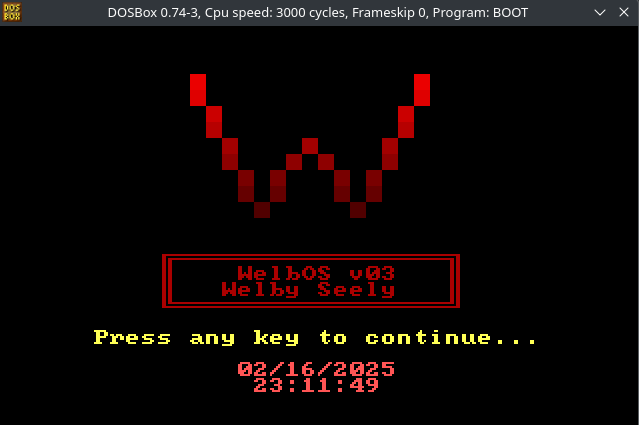
\includegraphics[width=\textwidth]{splash-screen} % Scales image to document width
        \caption{Custom splash screen, complete with logo and datetime in graphics mode}
        \label{fig:1}
    \end{figure}

    \begin{figure}[H]  % Ensures figure appears right here
        \centering
        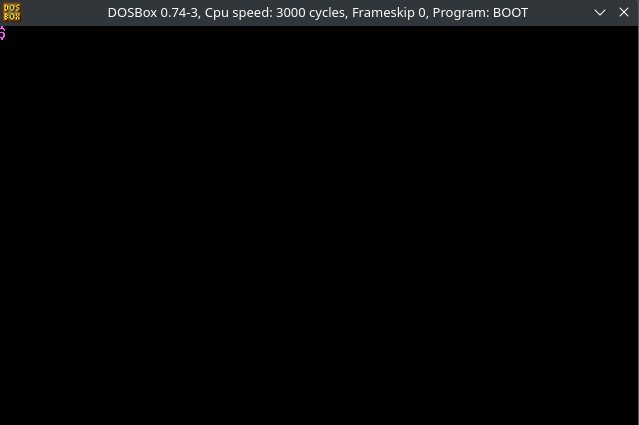
\includegraphics[width=\textwidth]{prompt} % Scales image to document width
        \caption{Prompt with \$ and a blinking cursor}
        \label{fig:2}
    \end{figure}

    \section{Appendix 1: Source Code}\label{sec:appendix_1}
    \begin{lstlisting}[caption={os623V03.asm listing}, captionpos=t]
        bits 16
BIOS_VIDEO          equ 0x10
DISPLAY_FUN         equ 0x13

FUN_VIDEO_MODE      equ 0x0000
VGA_MODE            equ 0x0013

BIOS_FLOPPY         equ 0x0013
READ_SECTORS        equ 0x0002

VGA_DISPLAY_WIDTH   equ 320
DISPLAY_WIDTH       equ 80
DISPLAY_HEIGHT      equ 25
VGA_TXT_DISP_WIDTH  equ 40
VGA_TXT_DISP_HEIGHT equ 25
MESSAGE_ROW         equ VGA_TXT_DISP_HEIGHT / 2 + 3
LINE_ROW_TOP        equ MESSAGE_ROW - 1
LINE_ROW_NAME       equ MESSAGE_ROW + 1
LINE_ROW_BOTTOM     equ LINE_ROW_NAME + 1
LINE_ROW_ANYKEY     equ LINE_ROW_BOTTOM + 2
TEXT_MODE           equ 0x03
MAGENTA_BLACK       equ 0x0D
WHITE_BLACK         equ 0x0F
RED_BLACK           equ 0x04
YELLOW_BLACK        equ 0x0E
LIGHT_RED           equ 0x0C

BOX_LENGTH          equ 19
ANYKEY_LENGTH       equ 28
BITMAP_LENGTH       equ 18
SHADE_COUNT         equ 9

; ext procedures
ANIMATE_LOGO_SEG equ 0x0001
ANIMATE_LOGO_OFF equ 0x2345

%define CENTER_TXT(len) ((DISPLAY_WIDTH - len) / 2)
%define CENTER_VGA_TXT(len) ((VGA_TXT_DISP_WIDTH - len) / 2)

org 0x7c00
jmp short start
nop

bsOEM       db "WelbOS v03"         ; OEM String

start:
    ; Inputs: cylinder, sector, head, segment, offset.
    push 1
    push 2
    push 0
    push ANIMATE_LOGO_SEG
    push ANIMATE_LOGO_OFF
    call load_sector

    push 1
    push 5
    push 0
    push 0x0002
    push 0x3456
    call load_sector

    call clear_screen

    mov ax, FUN_VIDEO_MODE + VGA_MODE
    int BIOS_VIDEO
    call set_red_gradient_palette

    push RED_BLACK
    push BOX_LENGTH
    push welbos
    push MESSAGE_ROW
    push CENTER_VGA_TXT(BOX_LENGTH)
    call print

    push RED_BLACK
    push BOX_LENGTH - 1               ; Repeat count
    push CENTER_VGA_TXT(BOX_LENGTH)   ; Column
    push LINE_ROW_TOP                 ; Row
    push topline                      ; Address of 3-tuple
    call draw_line

    push RED_BLACK
    push BOX_LENGTH
    push name
    push LINE_ROW_NAME
    push CENTER_VGA_TXT(BOX_LENGTH)
    call print

    push RED_BLACK
    push BOX_LENGTH - 1       ; Repeat count
    push CENTER_VGA_TXT(BOX_LENGTH)   ; Column
    push LINE_ROW_BOTTOM     ; Row
    push bottomline             ; Address of 3-tuple
    call draw_line

    push YELLOW_BLACK
    push ANYKEY_LENGTH
    push anykey
    push LINE_ROW_ANYKEY
    push CENTER_VGA_TXT(ANYKEY_LENGTH)
    call print

    ;push WHITE_BLACK
    ;push VGA_TXT_DISP_WIDTH - 1       ; Repeat count
    ;push 0   ; Column
    ;push LINE_ROW_ANYKEY + 2          ; Row
    ;push blockline                    ; Address of 3-tuple
    ;call draw_line

    call ANIMATE_LOGO_SEG:ANIMATE_LOGO_OFF
    call 0x0002:0x3456

    ; set segment to 2
    push 2
    pop ds

    push ax ;save for second call

    push LIGHT_RED
    push 10
    push ax
    push LINE_ROW_ANYKEY + 2
    push CENTER_VGA_TXT(10)
    call print

    pop ax  ; restore

    push LIGHT_RED
    push 8
    add ax, 10
    push ax
    push LINE_ROW_ANYKEY + 3
    push CENTER_VGA_TXT(8)
    call print

    ; restore segment
    push 0
    pop ds

    ; Wait for key press
    mov ah, 0x00
    int 0x16

    ; Switch back to text mode (80x25)
    mov ax, 0x0003
    int BIOS_VIDEO

    call clear_screen

    push MAGENTA_BLACK
    push 1
    push prompt_sym
    push 0
    push 0
    call print

    call set_cursor_pos



draw_line:
    push bp
    mov bp, sp

    ;left edge
    push word [bp + 12]
    push 1
    mov si, [bp + 4]
    push si
    mov si, [bp + 6]
    push si
    mov si, [bp + 8]
    push si
    call print

    ; set up middle loop
    mov ax, 1                           ; break when == to cx
draw_line_middle:
    mov cx, [bp + 10]
    cmp ax, cx
    je draw_line_right
    push ax

    push word [bp + 12]
    push 1
    mov si, [bp + 4]
    inc si
    push si
    mov si, [bp + 6]
    push si
    mov si, [bp + 8]
    add si, ax
    push si
    call print

    pop ax
    inc ax
    jmp draw_line_middle

draw_line_right:
    push word [bp + 12]
    push 1
    mov si, [bp + 4]
    add si, 2
    push si
    mov si, [bp + 6]
    push si
    add ax, [bp + 8]                    ; rightmostposition
    push ax
    call print

    pop bp
    ret 10


set_cursor_pos:
    mov ah, 0x02        ; BIOS function: set cursor position
    mov bh, 0x00        ; Page number (0)
    mov dh, 0x00        ; Row (0)
    mov dl, 0x01        ; Column (1)
    int BIOS_VIDEO
    ret

set_red_gradient_palette:
    mov dx, 0x3C8   ; VGA color index port
    mov al, 32      ; Start setting colors from index 32
    out dx, al
    inc dx          ; Now dx = 0x3C9 (RGB color data port)

    mov cx, 9       ; 9 shades for 9 rows
    mov si, red_shades
next_color:
    mov al, [si]    ; Load Red intensity
    out dx, al      ; Set Red value
    xor al, al      ; Set Green=0
    out dx, al
    out dx, al      ; Set Blue=0
    inc si
    loop next_color
    ret

; -----------------------------------------------------------------------------
; Function: clear_screen
; Description: Clears and resets the screen.
; Inputs: None.
; Outputs: None.
; Modifies:
;   - AX, BX, CX, DX
; Calls:
;   - BIOS interrupt 0x10, function 0x06.
; -----------------------------------------------------------------------------
clear_screen:
    mov ah, 0x06            ; BIOS scroll (function 06h)
    mov al, 0               ; Scroll all lines
    mov bh, WHITE_BLACK         ; Attribute
    mov ch, 0               ; Upper-left row
    mov cl, 0               ; Upper-left column
    mov dh, 24              ; Lower-right row
    mov dl, 79              ; Lower-right column
    int BIOS_VIDEO          ; BIOS video interrupt
    ret

; -----------------------------------------------------------------------------
; Function: load_sector
; Description: Loads sector 37 into memory.
; Inputs: cylinder, sector, head, segment, offset.
; Outputs: None.
; Modifies:
;   - AX, BX, CX, DX, EX
; Calls:
;   - BIOS interrupt 0x13, function 0x02.
; -----------------------------------------------------------------------------
load_sector:
    push bp
    mov bp, sp

	mov bx, [bp + 6]            ; segment (can't move immediate into segment register)
	mov es, bx                  ; segment
	mov bx, [bp + 4]            ; offset
	mov ah, READ_SECTORS        ; function
	mov al, 1                   ; number of sectors to read
	mov ch, [bp + 12]           ; cylinder number (10 bits, upper two bits are 6 and 7 of CL)
	mov cl, [bp + 10]           ; sector number (and upper two of cylinder)
	mov dh, [bp + 8]            ; head (usually same as side)
	mov dl, 0                   ; driver number
	int BIOS_FLOPPY

	pop bp
	ret 5

; -----------------------------------------------------------------------------
; Function: print
; Description: Prints a string to the console.
; Inputs:
;   - [sp+4] Column position to begin writing the string.
;   - [sp+6] Row position to begin writing the string.
;   - [sp+8] Memory address location of the string.
;   - [sp+10] Length of the string.
;   - [sp+12] Attribute.
; Outputs: None.
; Modifies:
;   - AX, BX, CX, DX
; Calls:
;   - BIOS interrupt 0x10, function 0x13.
; -----------------------------------------------------------------------------
print:
    push bp ; save bp for the return
    mov  bp, sp ; update bp to create a new "stack frame"

    mov bl, [bp+12]        ; Attribute (lightgreen on black)
    mov cx, [bp+10]        ; length of the string
    mov si, [bp+8]         ; address of the string
    mov dh, [bp+6]         ; row position
    mov dl, [bp+4]         ; column position

    ; We need ES:BP provides the pointer to the string - load the data segment (DS) base into ES
    push ds
    pop es

    mov  ah, DISPLAY_FUN    ; BIOS display string (function 13h)
    mov  al, 0              ; Write mode = 1 (cursor stays after last char
    mov  bh, 0              ; Video page
    mov  bp, si             ; Put offset in BP (ES:BP points to the string)
    int  BIOS_VIDEO

    pop bp                 ; Restore stack frame
    ret 10

topline             db 0xC9
                    db 0xCD
                    db 0xBB
bottomline          db 0xC8
                    db 0xCD
                    db 0xBC
blockline           db 0xDE
                    db 0xDC
                    db 0xDD
welbos              db 0xBA, `    WelbOS v03   `, 0xBA
welboslen           equ ($ - welbos)
name                db 0xBA, `   Welby Seely   `, 0xBA
namelen             equ ($ - name)
anykey              db "Press any key to continue..."
anykeylen           equ ($ - anykey)
prompt_sym          db "$"
red_shades db 58, 55, 50, 45, 40, 35, 30, 25, 20; Bright to dark red
; Pad to 512 bytes for an MBR:
padding times 510 - ($ - $$) db 0

; Optional boot signature:
bootSig db 0x55, 0xAA
    \end{lstlisting}

    \begin{lstlisting}[caption={loaderV03.asm listing}, captionpos=t]
        bits 16
VGA_DISPLAY_WIDTH   equ 320
SCALING_FACTOR      equ 0x8
LOGO_START_X        equ (VGA_DISPLAY_WIDTH - (16 * SCALING_FACTOR)) / 2
LOGO_START_Y        equ (200 - (9 * SCALING_FACTOR)) / 2 -40

org 0x2345
animate_logo:
    push ds
    push cs
    pop ds
    push LOGO_START_X
    push LOGO_START_Y
    call draw_logo
    pop ds
    retf

draw_logo:
    push bp
    mov bp, sp

    mov ax, [bp + 4]
    mov cx, VGA_DISPLAY_WIDTH
    mul cx
    add ax, [bp + 6]
    mov di, ax

    mov ax, 0xA000     ; memory mapped I/O segment for VGA
    mov es, ax

    mov si, w_bitmap   ; source bitmap start address

    mov dx, 9                  ; logical row that we're calculating
    push SCALING_FACTOR
draw_rows:
    mov bx, 9
    sub bx, dx                 ; determine color for this row
    mov bl, [row_colors + bx]  ; store row color in BL (or AL, but we’ll need AL soon)
    mov ax, [si]               ; retrieve pixels for this row

    ; Process 16 pixels
    mov cx, 16
draw_row:
    shl ax, 1          ; Shift left (test MSB of AX)
    jnc skip_column

    push cx
    push ax
    mov cx, SCALING_FACTOR
    mov al, bl
    rep stosb
    pop ax
    pop cx
    jmp next_column
skip_column:
    add di, SCALING_FACTOR
next_column:
    loop draw_row

scale_vertically:
    add di, 320 - 16 * SCALING_FACTOR ; Move to next VGA row
    pop cx
    dec cx
    cmp cx, 0
    jz next_source_row
    push cx
    jmp draw_rows
next_source_row:
    add si, 2
    dec dx
    jz logo_done
    push SCALING_FACTOR
    jmp draw_rows
logo_done:
    pop bp
    ret 4

w_bitmap db 02h, 80h
         db 02h, 80h
         db 04h, 40h
         db 04h, 40h
         db 08h, 21h
         db 88h, 22h
         db 50h, 14h
         db 50h, 14h
         db 20h, 08h
; Row color table, from top to bottom row
row_colors db 32, 33, 34, 35, 36, 37, 38, 39, 40  ; Use only custom red shades

    \end{lstlisting}

    \begin{lstlisting}[caption={datetimeV03.asm listing}, captionpos=t]
        %macro makedt 4
	mov bh,%1 			;dh/dl/chcl
	shr bh,4
	add bh,30h 			;add 30h to convert to ascii
	mov [%2 + %3],bh
	mov bh,%1
	and bh,0fh
	add bh,30h
	mov [%2 + %4],bh
%endmacro

bit16
org 0x3456

    push ds
    push cs
    pop ds

	mov ah,04h	 ;function 04h (get RTC date)
	int 1Ah		;BIOS Interrupt 1Ah (Read Real Time Clock)

	makedt dh, dtfld, 0, 1  ; month
	makedt dl, dtfld, 3, 4  ; day
	makedt ch, dtfld, 6, 7  ; century
	makedt cl, dtfld, 8, 9  ; year

	mov ah,02h
	int 1Ah

	makedt ch, tmfld, 0, 1  ; hours
	makedt cl, tmfld, 3, 4  ; minutes
	makedt dh, tmfld, 6, 7  ; seconds
	lea ax, [dtfld]
	pop ds
	retf

dtfld: db '00/00/0000'
tmfld: db '00:00:00'
    \end{lstlisting}

    \begin{lstlisting}[caption={Makefile listing}, captionpos=t]
        ##################################################
# Makefile of os623V0x.asm (x=[1,2,3])
##################################################

VER			= V03
ASM			= nasm
ASMFLAGS		= -f bin
IMG			= a.img

MBR			=  os623V.asm
MBR_SRC		= $(subst V,$(VER),$(MBR))
MBR_BIN		= $(subst .asm,.bin,$(MBR_SRC))

DATA_SRC	=  loaderV03.asm
DATA_BIN	=  data.bin

DATE_SRC	=  datetimeV03.asm
DATE_BIN	=  date.bin

.PHONY : everything

.PHONY : all everything clean reset blankimg

all: everything

everything : $(MBR_BIN) $(DATA_BIN) $(DATE_BIN)
 ifneq ($(wildcard $(IMG)), )
 else
		dd if=/dev/zero of=$(IMG) bs=512 count=2880
 endif

		dd if=$(MBR_BIN) of=$(IMG) bs=512 count=1 conv=notrunc
		dd if=$(DATA_BIN) of=$(IMG) bs=512 count=1 seek=37 conv=notrunc
		dd if=$(DATE_BIN) of=$(IMG) bs=512 count=1 seek=40 conv=notrunc

$(MBR_BIN) : $(MBR_SRC)
#	nasm -f bin $< -o $@
	$(ASM) $(ASMFLAGS) $< -o $@

$(DATA_BIN) : $(DATA_SRC)
	$(ASM) $(ASMFLAGS) $< -o $@

$(DATE_BIN) : $(DATE_SRC)
	$(ASM) $(ASMFLAGS) $< -o $@

clean :
	rm -f $(MBR_BIN) $(DATA_BIN)

reset:
	rm -f $(MBR_BIN) $(DATA_BIN) $(IMG)

blankimg:
	dd if=/dev/zero of=$(IMG) bs=512 count=2880
    \end{lstlisting}

\end{document}
